%% LaTeX2e class for student theses
%% thesis.tex
%%
%% Karlsruhe University of Applied Sciences
%% Faculty of  Computer Science and Business Information Systems
%% Distributed Systems (vsys)
%%
%% Prof. Dr. Christian Zirpins
%% christian.zirpins@hs-karlsruhe.de
%%
%%
%% Version 0.2, 2017-11-15
%%
%% --------------------------------------------------------
%% | Derived from sdqthesis by Erik Burger burger@kit.edu |
%% --------------------------------------------------------

%% Available languages: english,ngerman
%% Available modes: draft,final (see README)
\documentclass[ngerman,draft]{vsysthesis}
% Use space between paragraphs
%\KOMAoption{parskip}{half+}
\usepackage{acronym}

%% ---------------------------------
%% | Table related packages        |
%% ---------------------------------
\usepackage{tabularx}
\usepackage{multirow}
%% ---------------------------------
%% | Information about the thesis  |
%% ---------------------------------

%% Name of the author
\author{Armin Kunkel}

%% Title (and possibly subtitle) of the thesis
\title{Entwicklung eines Frameworks zur Integration von ActivityPub}

%% Type of the thesis
\thesistype{Bachelor Thesis}

%% Change the institute or subject area here, ``VSYS'' is default
% \myinstitute{Institute for \dots}

%% You can put a logo in the ``logos'' directory and include it here
% \grouplogo{myfile}

%% The reviewers are the professors that grade your thesis , ``Zirpins'' is default
%\reviewerone{Prof. A}
%% reviewer two (can be omitted)
%\reviewertwo{Prof. B}

%% The advisor is usually extern (can be omitted)
\advisorone{M. Sc. Robert Sch\"{a}fer}
% The second advisor (can be omitted)
%\advisortwo{Dipl.-Inform. D}


%% Please enter the start end end time of your thesis
\editingtime{
	\iflanguage{english}{01. December 2018}{01. Dezember 2018}
}{
	\iflanguage{english}{31. March 2019}{31. M\"{a}rz 2019}
}

\settitle

%% --------------------------------
%% | Settings for word separation |
%% --------------------------------

%% Describe separation hints here.
%% For more details, see
%% http://en.wikibooks.org/wiki/LaTeX/Text_Formatting#Hyphenation
\hyphenation{
% me-ta-mo-del
}

%% --------------------------------
%% | Bibliography                 |
%% --------------------------------

%% Use biber instead of BibTeX, see README
\usepackage[style=numeric,backend=biber]{biblatex}
\addbibresource{thesis.bib}

%% Package for switching between languages
\usepackage{iflang}

%% Figures in a vertical bar and more..
\usepackage{subcaption}
%% --------------------------------
%% | Listings                     |
%% --------------------------------
\usepackage{xcolor}
\usepackage{listings}
\definecolor{mygreen}{rgb}{0,0.6,0}
\definecolor{mygray}{rgb}{0.5,0.5,0.5}
\definecolor{mymauve}{rgb}{0.58,0,0.82}
\definecolor{lightgray}{rgb}{.9,.9,.9}
\definecolor{darkgray}{rgb}{.4,.4,.4}
\definecolor{purple}{rgb}{0.65, 0.12, 0.82}

\lstset{ %
	backgroundcolor=\color{white}, % choose the background color; you must add \usepackage{color} or \usepackage{xcolor}
	basicstyle=\footnotesize, % the size of the fonts that are used for the code
	breakatwhitespace=false, % sets if automatic breaks should only happen at whitespace
	breaklines=true, % sets automatic line breaking
	captionpos=b, % sets the caption-position to bottom
	commentstyle=\color{mygreen}, % comment style
	escapeinside={\%*}{*)}, % if you want to add LaTeX within your code
	extendedchars=true, % lets you use non-ASCII characters; for 8-bits encodings only, does not work with UTF-8
	frame=single, % adds a frame around the code
	keepspaces=true, % keeps spaces in text, useful for keeping indentation of code (possibly needs columns=flexible)
	keywordstyle=\color{blue}, % keyword style
	% language=Octave, % the language of the code
	numbers=left, % where to put the line-numbers; possible values are (none, left, right)
	numbersep=5pt, % how far the line-numbers are from the code
	numberstyle=\tiny\color{mygray}, % the style that is used for the line-numbers
	rulecolor=\color{black}, % if not set, the frame-color may be changed on line-breaks within not-black text (e.g. comments (green here))
	showspaces=false, % show spaces everywhere adding particular underscores; it overrides 'showstringspaces'
	showstringspaces=false, % underline spaces within strings only
	showtabs=false, % show tabs within strings adding particular underscores
	stepnumber=1, % the step between two line-numbers. If it's 1, each line will be numbered
	stringstyle=\color{mymauve}, % string literal style
	tabsize=2, % sets default tabsize to 2 spaces
	title=\lstname % show the filename of files included with \lstinputlisting; also try caption instead of title
}

%define Javascript language
\lstdefinelanguage{JavaScript}{
	keywords={typeof, new, true, false, catch, function, return, null, catch, switch, var, if, in, while, do, else, case, break},
	keywordstyle=\color{blue}\bfseries,
	ndkeywords={class, export, boolean, throw, implements, import, this},
	ndkeywordstyle=\color{darkgray}\bfseries,
	identifierstyle=\color{black},
	sensitive=false,
	comment=[l]{//},
	morecomment=[s]{/*}{*/},
	commentstyle=\color{purple}\ttfamily,
	stringstyle=\color{red}\ttfamily,
	morestring=[b]',
	morestring=[b]"
}

\colorlet{punct}{red!60!black}
\definecolor{background}{HTML}{EEEEEE}
\definecolor{delim}{RGB}{20,105,176}
\colorlet{numb}{magenta!60!black}

\lstdefinelanguage{json}{
	basicstyle=\normalfont\ttfamily,
	numbers=left,
	numberstyle=\scriptsize,
	stepnumber=1,
	numbersep=8pt,
	showstringspaces=false,
	breaklines=true,
	frame=lines,
	backgroundcolor=\color{background},
	literate=
	*{0}{{{\color{numb}0}}}{1}
	{1}{{{\color{numb}1}}}{1}
	{2}{{{\color{numb}2}}}{1}
	{3}{{{\color{numb}3}}}{1}
	{4}{{{\color{numb}4}}}{1}
	{5}{{{\color{numb}5}}}{1}
	{6}{{{\color{numb}6}}}{1}
	{7}{{{\color{numb}7}}}{1}
	{8}{{{\color{numb}8}}}{1}
	{9}{{{\color{numb}9}}}{1}
	{:}{{{\color{punct}{:}}}}{1}
	{,}{{{\color{punct}{,}}}}{1}
	{\{}{{{\color{delim}{\{}}}}{1}
	{\}}{{{\color{delim}{\}}}}}{1}
	{[}{{{\color{delim}{[}}}}{1}
	{]}{{{\color{delim}{]}}}}{1},
}

\lstset{
	language=JavaScript,
	extendedchars=true,
	basicstyle=\footnotesize\ttfamily,
	showstringspaces=false,
	showspaces=false,
	numbers=left,
	numberstyle=\footnotesize,
	numbersep=9pt,
	tabsize=2,
	breaklines=true,
	showtabs=false,
	captionpos=b
}
\lstset{
	language=json,
	extendedchars=true,
	basicstyle=\footnotesize\ttfamily,
	showstringspaces=false,
	showspaces=false,
	numbers=left,
	numberstyle=\footnotesize,
	numbersep=9pt,
	tabsize=2,
	breaklines=true,
	showtabs=false,
	captionpos=b
}

%% --------------------------------
%% | Glossaries                   |
%% --------------------------------

%% Use glossaries (optional)
\makeglossaries
%% Load glossary definitions from file
\loadglsentries{glossentries.tex}
%% ====================================
%% ====================================
%% ||                                ||
%% || Beginning of the main document ||
%% ||                                ||
%% ====================================
%% ====================================
\begin{document}
% set text color to black
%\color{black}\global\let\default@color\current@color

%% Set PDF metadata
\setpdf

%% Set the title
\maketitle

%% The Preamble begins here
\frontmatter

%% LaTeX2e class for student theses: Declaration of independent work
%% sections/declaration.tex
%%
%% Karlsruhe University of Applied Sciences
%% Faculty of  Computer Science and Business Information Systems
%% Distributed Systems (vsys)
%%
%% Prof. Dr. Christian Zirpins
%% christian.zirpins@hs-karlsruhe.de
%%
%%
%% Version 0.2, 2017-11-15
%%
%% --------------------------------------------------------
%% | Derived from sdqthesis by Erik Burger burger@kit.edu |
%% --------------------------------------------------------


\thispagestyle{empty}
\null\vfill
\noindent\hbox to \textwidth{\hrulefill}
\iflanguage{english}{I declare that I have developed and written the enclosed
thesis completely by myself, and have not used sources or means without
declaration in the text.}{Ich versichere wahrheitsgemäß, die Arbeit
selbstständig angefertigt, alle benutzten Hilfsmittel vollständig und genau
angegeben und alles kenntlich gemacht zu haben, was aus Arbeiten anderer
unverändert oder mit Änderungen entnommen wurde.}%



%% ---------------------------------------------
%% | Replace PLACE and DATE with actual values |
%% ---------------------------------------------
\textbf{Karlsruhe, \today}
\vspace{1.5cm}

\dotfill\hspace*{8.0cm}\\
\hspace*{2cm}(\theauthor)
\cleardoublepage


\setcounter{page}{1}
\pagenumbering{roman}

%% ----------------
%% |   Abstract   |
%% ----------------

%% For theses written in English, an abstract both in English
%% and German is mandatory.
%%
%% For theses written in German, a German abstract is sufficient.
%%
%% The text is included from the following files:
%% - chapters/abstract

\includeabstract

%% ------------------------
%% |   Table of Contents  |
%% ------------------------
\tableofcontents
\listoffigures
\listoftables

%% ------------------------
%% | Glossary/Acronyms    |
%% ------------------------

% print glossary (optional)
%\printglossary[style=altlist,title=Glossar]

% print acronyms (optional)
%\printglossary[style=long,type=\acronymtype]

\chapter{Abkürzungsverzeichnis}

\begin{acronym}[swwg]
	\acro{SWWG}{Social Web Working Group}
	\acro{W3C}{World Wide Web Consortium}
	\acro{DSA}{Digital Signature Algorithm}
	\acro{OWP}{Open Web Platform}
	\acro{RSA}{Rivest-Shamir-Adleman}
	\acro{API}{Application Programming Interface}
\end{acronym}

%% -----------------
%% |   Main part   |
%% -----------------

\mainmatter

%% LaTeX2e class for student theses
%% sections/content.tex
%%
%% Karlsruhe University of Applied Sciences
%% Faculty of  Computer Science and Business Information Systems
%% Distributed Systems (vsys)
%%
%% Prof. Dr. Christian Zirpins
%% christian.zirpins@hs-karlsruhe.de
%%
%%
%% Version 0.2, 2017-11-15
%%
%% --------------------------------------------------------
%% | Derived from sdqthesis by Erik Burger burger@kit.edu |
%% --------------------------------------------------------
\chapter{ 
	\iflanguage{english}{Introduction}{Einleitung}
}
\label{ch:Introduction}
\iflanguage{english}{
	\todo{- Justification of this work}
	Centralization of data and trust in individual instances is ubiquitous today. In the Internet there is a wealth of social networks such as Facebook, Twitter, Google+, Instagram or Pinterest which mostly retain the right to the data you get from their users and last but not least sell this data for advertising purposes. It is also easier for criminals and secret services to access the entire database, since centralised networks usually also have a central database or access point. When the access to this central point is reached, the whole database can be read.\\
	
	What does decentralized mean? In politics, decentralization \glqq is the transfer of central government tasks to subnational or subsidiary level(s)\grqq\cite{wikipedia-decentralization-politics}. In the energy industry, one speaks of \glqq decentralized power generation\grqq if the power is also generated at the places where it is consumed. An example of this would be a hydroelectric power plant that supplies electricity to the surrounding villages or cities\cite{wikipedia-decentralization-energy}. In computer science, decentralization means the distribution of data over several independent servers. \\
	
	By allocating tasks to sub-national or subsidiary levels, the central government level is relieved of its burden and thus has more resources for other tasks. When hydroelectric power plants are built close to villages and towns, there is no need to transport electricity over long distances, which reduces the loss of electricity when it is transported over the power grid. Decentralisation of social networks brings various advantages. One advantage is the scalability of decentralized social networks. By adding more instances, new resources can be made available to the network. Another advantage is that there is no central control body that can be corrupted by criminals, economic lobbyists or government authorities.\\
	
	% - Goal of the work
	The aim of the work is to implement the distributed server-to-server protocol as a prototype and to test the security standards for the ActivityPub protocol recommended by the \gls{w3c} community. In addition, the work should give an overview of the basics of the protocol and how the relevant components are to be understood. The security standards used relate to the authentication of the client against the server and additionally the server to each other, as well as ensuring the manipulation-free transmission of content.\\

}{
	%	- 	Rechtfertigung der Arbeit
	Zentralisierung von Daten und das Vertrauen auf einzelne Instanzen ist heutzutage allgegenwärtig. Im Internet gibt es eine Fülle an sozialen Netzwerken wie Facebook, Twitter, Google+, Instagram oder Pinterest die zumeist das Recht an den Daten, die Sie von ihren Nutzer bekommen, behalten und nicht zuletzt diese Daten auch verkaufen für z. B. Werbezwecke. Für Kriminelle sowie Geheimdienste ist es außerdem leichter an die gesamte Datenbank zu kommen, da bei zentralisierten Netzwerken meist auch eine zentrale Datenbank, bzw. ein zentraler Zugriffspunkt, vorhanden ist. Wenn der Zugriff auf diesen zentralen Punkt erreicht ist kann die ganze Datenbank ausgelesen werden.\\
	
	Was bedeutet nun dezentral? In der Politik wird unter Dezentralisierung \glqq die Übertragung zentral staatlicher Aufgaben auf subnationale oder subsidiäre Ebene(n) verstanden\grqq\cite{wikipedia-dezentralisierung-politik}. In der Energiewirtschaft spricht man von einer \glqq dezentralen Stromerzeugung\grqq, wenn der Strom an den Stellen wo er verbraucht auch erzeugt wird. Ein Beispiel hierfür wäre ein Wasserkraftwerk, dass den Strom für die umgebenen Dörfer oder Städte liefert\cite{wikipedia-dezentralisierung-energie}. In der Informatik versteht man unter Dezentralisierung das verteilen von u. a. Daten über mehrere unabhängige Server hinweg.\\
	
	Durch die Verteilung der Aufgaben auf sub-nationale oder subsidiäre Ebene wird die zentral staatliche Ebene entlastet und hat somit mehr Ressourcen für andere Aufgaben. Beim Errichten von Wasserkraftwerken nahe an Dörfern und Städten entfällt der Transport des Stroms über größere Distanzen und somit verringert sich der Verlust beim Transport über das Stromnetz. Dezentralisieren von sozialen Netzwerken bring verschiedene Vorteile mit sich. Ein Vorteil ist die Skalierbarkeit bei dezentralen sozialen Netzwerken. Durch das hinzufügen weiterer Instanzen können dem Netzwerk neue Ressourcen bereitgestellt werden. Ein weiterer Vorteil liegt darin, dass keine zentrale Kontrollinstanz vorhanden ist welche korrumpiert werden kann, sei es durch Kriminelle, wirtschaftliche Interessenvertreter oder staatliche Autoritäten.\\
	
	%	- 	Ziel der Arbeit
	Ziel der Arbeit ist es die Implementierung des förderierten Server-zu-Server Protokolls als Prototyp vorzunehmen und die bis dato von der \gls{w3c} Gemeinschaft empfohlenen Sicherheitsstandards für das ActivityPub Protokoll zu prüfen. Es soll die Frage geklärt werden ob HTTP- und Linked Data Signaturen bestmöglich dafür geeignet sind, die sichere Kommunikation zu gewährleisten anhand eines Vergleichs der beiden Verfahren. Darüber hinaus soll die Arbeit einen Überblick über die Grundlagen des Protokolls geben und wie die relevanten Bestandteile zu verstehen sind. In diesem Zusammenhang ist mit \glqq sicher\grqq~die authentische und manipulationsfreie Übertragung der Server untereinander gemeint.\\
	% Schutzziele
	%	- 	Abgrenzung des Themas und Themenbezogenen Definitionen
		
	%	- 	Geschichte und Stand der Forschung:
	\todo{Firma vorstellen}
}

\section{Motivation}
\label{sec:Introduction:Motivation}
\iflanguage{english}{
	With central social networks, e.g. Facebook, the company has control over data. Due to decentralization, data remains with the individual instances of the social network. Although the databases in central networks can be distributed and the network can also be decentralized, the data still belongs to one company. In addition, central social networks cannot easily exchange content with other networks. With a protocol like ActivityPub, distributing and accessing content and sharing activities across multiple social networks is made possible.\\
	
	ActivityPub consists of two parts. The client-to-server protocol, also called \glqq Social API\grqq~, and the promoted server-to-server protocol. Through the ActivityPub \gls{w3c} recommendation in early 2018 and the \gls{swwg} working group of the \gls{w3c} and others, the dissemination of the protocol is promoted. \\
	
	The network effect is a term derived from economics. One example is the telephone network. The more people own a phone, the greater the benefit for each individual phone owner\cite{network effect}. Transferred to ActivityPub this means as much as: \glqq The more networks implement the standard, the greater the benefit for a single network and ultimately for individual users\grqq.\\
	
	%In the following, a brief distinction is made between the two terms decentralized and federated.\\
	
	Protocols such as \glqq Diaspora Federation and OStatus\grqq~provide access to decentralized social content and enable the publication of social content. The standard recommended in March last year by \gls{w3c} called \glqq ActivityPub\grqq~was developed on the basis of the knowledge in dealing with the OStatus and Pump.io protocol\cite{activityPub}.\\
	
	ActivityPub is like \glqq OStatus\grqq~a protocol for decentralized social networks and is examined in this Bachelor thesis.
}{
	Bei zentralen sozialen Netzwerken, z.B. Facebook, besitzt die Kontrolle über Daten das Unternehmen. Durch die Dezentralisierung bleiben Daten bei den einzelnen Instanzen des sozialen Netzwerkes. Die Datenbanken bei zentralen Netzwerken können zwar verteilt sein und auch das Netzwerk könnte dezentral angelegt sein, trotzdem gehören die Daten einem Unternehmen. Außerdem können bei zentralen sozialen Netzwerken nicht ohne weiteres Inhalte mit anderen Netzwerken ausgetauscht werden. Mit einem Protokoll wie ActivityPub wird das Verteilen sowie der Zugriff auf Inhalte und der Austausch von Aktivitäten über mehrere soziale Netzwerke hinweg ermöglicht.\\
	
	ActivityPub besteht aus zwei Teilen. Dem Client-zu-Server Protokoll, auch \glqq Social API\grqq~genannt, und dem förderierten Server-zu-Server Protokoll. Durch die ActivityPub \gls{w3c} Empfehlung Anfang 2018 und die \gls{swwg} Arbeitsgruppe des \gls{w3c} sowie weiteren, wird die Verbreitung des Protokolls vorangebracht.\\
	
	Der Netzwerkeffekt ist ein aus der Volkswirtschaftslehre stammender Begriff. Als Beispiel sei das Telefonnetz genannt. Umso mehr Leute ein Telefon besitzen, umso höher ist der Nutzen für jeden einzelnen Telefon Besitzer\cite{netzwerkeffekt}. Übertragen auf ActivityPub bedeutet das soviel wie: \glqq Je mehr Netzwerke den Standard implementieren, desto höher ist der Nutzen für ein einzelnes Netzwerk und im Endeffekt für die einzelnen Nutzer\grqq.\\
	%Der Grundgedanke des World Wide Web nach Tim Beners Lee war es ein offenes und freies Web zu schaffen um Wissen für die Allgemeinheit zugänglich zu machen. \todo{Quelle: Web-Report stelle suchen}
	%Im folgenden wird kurz unterschieden zwischen den zwei Begriffen dezentral und förderiert.\\
	
	
	Protokolle wie \glqq Diaspora Federation und OStatus\grqq~bieten den Zugriff auf dezentral gespeicherte soziale Inhalte und ermöglichen das veröffentlichen von sozialen Inhalten. Der im März letzten Jahres vom \gls{w3c} empfohlene Standard namens \glqq ActivityPub\grqq~wurde auf Basis des Wissens im Umgang mit dem OStatus und Pump.io Protokoll entwickelt\cite{activityPub}.\\ 
	\todo{Quelle für dezentralen Zugriff}
	
	ActivityPub ist wie \glqq OStatus\grqq~ein Protokoll für dezentrale soziale Netzwerke und wird in dieser Bachelor Arbeit untersucht.
}

%\section{Unterschied zentraler sozialer zu dezentralen sozialen Netzwerken}

%%% LaTeX2e class for student theses
%% sections/content.tex
%%
%% Karlsruhe University of Applied Sciences
%% Faculty of  Computer Science and Business Information Systems
%% Distributed Systems (vsys)
%%
%% Prof. Dr. Christian Zirpins
%% christian.zirpins@hs-karlsruhe.de
%%
%%
%% Version 0.2, 2017-11-15
%%
%% --------------------------------------------------------
%% | Derived from sdqthesis by Erik Burger burger@kit.edu |
%% --------------------------------------------------------

\chapter{Verwandte Protokolle}
	\iflanguage{english}{
		A network of networks is therefore referred to as a network interconnection, or \glqq federated network\grqq.\\
		
		A promotion is the association of something. Germany, for example, is a subsidised federal state linking 16 federal states. A network of networks is therefore referred to as a network interconnection, or \glqq federated network\grqq.\\
		
		\glqq Fediverse\grqq~is a suitcase word from \glqq Federated\grqq~and \glqq Universe\grqq. Historically, the term has only included microblogging platforms that support the OStatus protocol. More about OStatus \textbf{S. \ref{sub:ostatus}}. Meanwhile the Fediverse contains more than just microblogging platforms like Mastodon\footnote{\url{https://mastodon.social/about}} but also social networks (e.g. GNU Social\footnote{\url{https://gnu.io/social/}}), as well as \glqq Video hosting\grqq~(PeerTube\footnote{\url{https://joinpeertube.org/en/}}),\glqq Content publishing\grqq~ Platforms, like Wordpress, and many more.\cite{fediverse}
		
		The \glqq Fediverse\grqq~is all about free (open source) software instead of commercial products. You can also choose which administrator you want to give control over your data instead of relying on a single instance.\cite{fediverse}\\
		
		According to the Fediverse Network Report 2018, which is available online, the total number of reachable instances has increased from 2,756 to 4,340. This corresponds to growth of 58\%. The number of users rose from 1,786,036 to 2,474,601 (39\%). Further details can be found in the Network Report. It should be added that the network report is incomplete and may contain bugs.\cite{fediverse-report}\\
	}{
		Zu Beginn dieses Kapitels wird das Wort Fediverse etwas näher definiert und erläutert worum es sich dabei handelt. Im Anschluss werden mehrere Protokolle die, sowie auch ActivityPub, zum Fediverse gehören vorgestellt.\\
		
		Als erstes soll der Begriff \glqq förderiertes Netzwerk\grqq~von Förderation hergeleitet werden. Unter einer Förderation versteht man den Verbund von etwas. Deutschland ist z. B. ein förderierter Bundesstaat, welcher 16 Bundesländern verbindet. Ein Verbund von Netzwerken wird demnach als Netzwerkverbund, oder auch \glqq förderiertes Netzwerk\grqq,~bezeichnet.\\
		
		\glqq Fediverse\grqq~ist ein Kofferwort aus \glqq Federated\grqq~und \glqq Universe\grqq. Historisch gesehen beinhaltete der Begriff nur Microblogging Plattformen die das OStatus Protokoll unterstützen. Mehr zu OStatus \textbf{S. \ref{sub:ostatus}}. Mittlerweile beinhaltet das Fediverse mehr als nur Microblogging Plattformen wie Mastodon\footnote{\url{https://mastodon.social/about}} und GNU Social\footnote{\url{https://gnu.io/social/}}, sondern auch soziale Netzwerke, sowie \glqq Video hosting\grqq~(PeerTube\footnote{\url{https://joinpeertube.org/en/}}),\glqq Content publishing\grqq~Plattformen, wie Wordpress, und viele weitere.\cite{fediverse}\\
		
		Im \glqq Fediverse\grqq~dreht sich alles um freie (Open Source) Software anstelle von kommerziellen Produkten. Zudem kann ausgesucht werden welchem Administrator man die Kontrolle über seine Daten geben möchte, anstatt auf eine einzelne Instanz vertrauen zu müssen.\cite{fediverse} Ein weiterer wichtiger Aspekt ist das verbünden von Netzwerken über Protokolle wie OStatus oder Pump.io. Somit kann ein verteiltes soziales Netzwerk durch die Implementierung eines dieser Protokolle zum förderierten sozialen Netzwerk werden.\\
		\todo{indirektes online Zitat!!!}
		
		Laut dem Fediverse Netzwerkreport 2018, welcher online zur Verfügung steht, hat sich die Gesamtanzahl der erreichbaren Instanzen von 2.756 auf 4.340 erhöht. Dies entspricht einem Wachstum von 58\%. Die Nutzeranzahl ist von 1.786.036 auf 2.474.601 gestiegen (39\%). Weitere Details sind im Netzwerk Report nachzulesen. Es ist hinzuzufügen das der Netzwerkreport unvollständig ist und Fehler beinhalten kann.\cite{fediverse-report}\\	
		
			\todo{Vergleich der Vor- und Nachteile der Protokolle}
		\section{OStatus}
		\label{sub:ostatus}
		Der OStatus Standard ist eine Sammlung von verschiedenen Protokollen wie Atom, Activity Streams, WebFinger und weiteren. Ausgelegt ist der Standard auf das empfangen und versenden von Status updates für förderierte Microblogging Dienste wie z. B. Mastodon und Friendica. Das Zusammenspiel mehrerer Protokolle ermöglicht den Austausch von Status updates in fast Echtzeit.
		\section{Diaspora}
		\label{sub:diaspora}
		Diaspora ist ein freier Web Server mit einer integrierten Implementierung eines verteilten sozialen Netzwerkes. In diesem Netzwerk wird ein Knoten als Pod bezeichnet. Die einzelnen Pods sind das, was das Diaspora Netzwerk ausmacht. Durch die integrierte Funktionalität zum sozialen Netzwerken kann auf dem Web Server aufsetzend eine eigene Applikation entwickelt werden.
		\section{Pump.io}
		\label{sub:pumpio}
		Der ActivityPub Standard wurde mit der gesammelten Erfahrung im Umgang mit dem Pump.io Protokoll entwickelt.
	}
%% LaTeX2e class for student theses
%% sections/content.tex
%%
%% Karlsruhe University of Applied Sciences
%% Faculty of  Computer Science and Business Information Systems
%% Distributed Systems (vsys)
%%
%% Prof. Dr. Christian Zirpins
%% christian.zirpins@hs-karlsruhe.de
%%
%%
%% Version 0.2, 2017-11-15
%%
%% --------------------------------------------------------
%% | Derived from sdqthesis by Erik Burger burger@kit.edu |
%% --------------------------------------------------------

\chapter{
	\iflanguage{english}{Basics for the secure implementation of decentralised social networks}{Grundlagen zur sicheren Umsetzung dezentraler sozialer Netzwerke}
}
\label{ch:fundamentals}
\iflanguage{english}{}{
	\todo{Allgemeine Grundlagen zu Sozialen Netzwerken/Social Media und deren Sicherheitsaspekte}
	\todo{Welche Klassen von Anwendungen und Implementierungen gibt es allgemein bei sozialen Netzwerken? Einordnen von ActivityPub!!}
	%\todo{AP Beschreibung in hinteren Teil des Grundlagenkapitels oder zu Beginn des 3. Kapitels}
	%Klassen von Anwendungen sowie Implementierungen erläutert.
	Dieses Kapitel gibt einen Überblick über allgemeine Grundlagen von sozialen Netzwerken. Es wird grob erläutert für was soziale Netzwerke gedacht sind; Der Unterschied zwischen zentralen, verteilen, dezentralen und förderierten sozialen Netzwerken herausgestellt sowie auf Sicherheitsaspekte eingegangen.\par
	
	Im Anschluss wird ein Kryptographie Unterkapitel eingeführt in dem die benötigten Verfahren für die sichere Umsetzung erläutert werden. Begonnen wird mit einer kurzen Einführung in Kryptographie. Darauf folgend wird kurz das RSA Verfahren sowie eine allgemeine Beschreibung von Signatur Algorithmen vorgenommen. HTTP Signaturen werden ausführlicher beschrieben, da diese bei der Implementierung des Prototypen verwendet wurden.\par 
	
	Darauf folgend wird der ActivityPub Standard eingeführt sowie eingeordnet, Bestandteile des Protokolls beschrieben, die Funktionsweise der Client-zu-Server sowie Server-zu-Server Kommunikation und zugehörige Standards kurz erläutert. Desweiteren wird auf die Authentifizierung und Datenintegrität bei ActivityPub eingegangen um damit folgende Fragen zu klären:
	\begin{itemize}
		\item Wie authentifiziert sich ein Benutzer gegenüber dem Server?
		\item Wie stellt man sicher, dass die übertragenen Daten unverändert angekommen sind?
	\end{itemize}
}
\section{
	\iflanguage{english}{General principles of social networks}{Allgemeine Grundlagen sozialer Netzwerke}		
}
In den Sozialwissenschaften versteht man unter einem sozialen Netzwerk mehrere Personen die miteinander wechselwirkend auf soziale weise interagieren. Die Informatik bildet soziale Netzwerke als Plattformen zum Aufbau und der Pflege von Beziehungen ab. Weiter gefasst können auch Mikroblogging-Dienste, Chat Software, Voice Chat-Programme u. s. w. zu sozialen Netzwerken gezählt werden, da auch die Möglichkeit geboten wird sozial miteinander zu interagieren\cite{wikipedia-social-network-sociology}.
	\begin{figure}[h]
		\begin{minipage}{\textwidth}
			\centering
			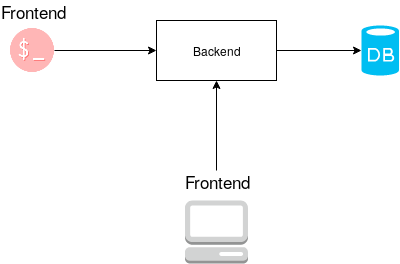
\includegraphics[scale=0.55]{figures/central-social-network.png}
			\label{fig:central-social-network}
			\caption{3 Tier Architektur}
		\end{minipage}
	\end{figure}
	Im Allgemeinen besteht ein soziales Netzwerk aus Softwaretechnischer Sicht aus 3 Komponenten, dies ist aber keine Prämisse. Der Nutzer benutzt das Netzwerk durch eine meist grafische Schnittstelle. Um Zugriff auf das Netzwerk zu erlangen benötigt der Nutzer ein \textit{\textbf{Frontend}}. Dies kann in grafischer Form oder als \gls{cli} zur Verfügung stehen. Über das Frontend kann der Nutzer sich nun mit seinen Anmeldeinformationen am \textit{\textbf{Backend}} anmelden und somit meist eine Sitzung eröffnen. Steht ein Web Interface zur Verfügung, werden Sitzungen oft über Clientseitige Cookie Speicherung aufrecht erhalten. Das Backend hat die Aufgabe eingehende Nutzeranfragen entsprechend zu beantworten und, falls autorisiert, die gewünschten Aufgaben auszuführen. Bei größeren sozialen Netzwerken fällt eine große Menge generierter Daten an die verwaltet werden müssen. Dafür wird meistens eine \textit{\textbf{Datenbank}} herangezogen die zumeist auch repliziert betrieben wird. An sich kann ein zentrales Netzwerk auch über den Einsatz von virtuellen Maschinen und Lastenverteilung verteilt oder dezentral sein. Beispielsweise könnte ein zentrales soziales Netzwerk Anfragen länderspezifisch an zuständige Instanzen des Netzwerks weiterleiten. Auch ist es Möglich die Daten länderspezifisch zu speichern und somit den Nutzern aus Deutschland andere Inhalte anzubieten als Nutzern aus der Schweiz.\par
	\subsection{
		\iflanguage{english}{Difference between centralised, decentralised and distributed social networks}{Unterschiedliche Klassen sozialer Netzwerke}
	}
	\label{sub:difference}
	\textit{Zentrale soziale Netzwerke} haben den Nachteil eines \glqq Single point of Failures\grqq. Fällt dieser Knoten aus, bricht das ganze Netzwerk zusammen. Zudem sind sie kaum Skalierbar. Ein Vorteil eines zentralen Netzwerks ist die schnelle Bereitstellbarkeit. Obwohl aus Sicht der Daten die meisten sozialen Netzwerke zentral sind, kann ihre Architektur intern sowohl verteilt als auch dezentral sein.\par
	
	\begin{figure}[!t] 
		\centering
		\begin{subfigure}[t]{0.4\linewidth}
			\centering
			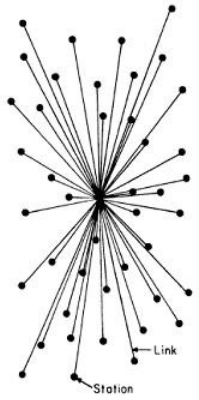
\includegraphics[width=0.4\linewidth]{figures/centralized-network.png}
			\caption{Zentrales soziale Netzwerk}
			\label{fig:central-network}
		\end{subfigure}
		\begin{subfigure}[t]{0.4\linewidth}
			\centering
			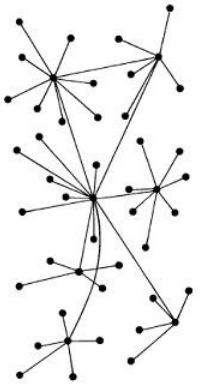
\includegraphics[width=0.4\linewidth]{figures/decentralized-network.png}
			\caption{Dezentrales soziale Netzwerk}
			\label{fig:decentral-network}
		\end{subfigure}
		\begin{subfigure}[t]{0.4\linewidth}
			\centering
			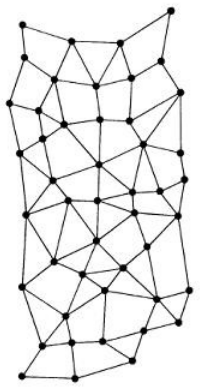
\includegraphics[width=0.4\linewidth]{figures/distributed-network.png}
			\caption{Verteilte soziale Netzwerk}
			\label{fig:distributed-network}
		\end{subfigure}
		\vspace{4pt}
		\quelle{(Zentrale, dezentrale, verteilte Systeme)}
		\caption{Klassen sozialer Netzwerke}
	\end{figure}\par

	In der obigen Abbildung ist ein zentrales Netzwerk gezeigt welches aus einem zentralen Knoten (Peer) und verschiedenen Blättern (Inhalten) besteht. Fällt der zentrale Knoten aus, kann auf die von diesem Netzwerk bereitgestellten Inhalte nicht mehr zugegriffen werden.\par
	
	Bei einem \textit{dezentralen sozialen Netzwerk} verhält sich das anders. Fällt ein Peer aus, kann auf die Inhalte aller weiterer Peers weiterhin zugegriffen werden. Zudem sind die Inhalte bei dezentralen Netzwerken auf die Peers verteilt anstatt das alle auf ein einer Instanz residieren.\par
	
	\textit{Verteilte soziale Netzwerke} verfügen zusätzlich über eine Middleware Schicht über die einzelne Peers kommunizieren können. Dadurch ist unter anderen eine leichte Skalierbarkeit gegeben, da eine weitere Instanz lediglich gestartet werden muss.\par
	
	Um die Inhalte verschiedener Netzwerke zu verbinden können mehrere soziale Netzwerke zu einem großen verbunden oder \glqq förderiert\grqq~werden. Dies kann über Protokolle und Standards wie OStatus und ActivityPub geschehen oder durch Netzwerkbrücken, im Sinne von Transformatoren, realisiert werden.\par
	\subsection{
		\iflanguage{english}{Security aspects of social networks}{Sicherheitsaspekte sozialer Netzwerke}
	}
	\todo{Authentifizierung Client gegenüber Server}
	\todo{Sicherstellen der Datenintegrität}
	\todo{Filterung auf Rechte (Nutzer bekommt nur das zu sehen, was er sehen darf)}\par
\section{
	\iflanguage{english}{cryptography}{Kryptographie}
}
\iflanguage{english}{}{
	\glqq Unter dem Begriff Kryptographie ist die Wissenschaft vom geheimen Schreiben zu verstehen\grqq\footnote{Dietmar Wätjen, 2018, S.1}. Man spricht von symmetrischer Verschlüsselung wenn eine Nachricht im Klartext vom Sender mit einem geheimen Schlüssel, welcher beiden Parteien bekannt ist, verschlüsselt und vom Empfänger, mit demselben Schlüssel, entschlüsselt wird\footnote{Vgl. Dietmar Wätjen, 2018, S.1}.\par
	\begin{figure}[h]
		\begin{minipage}{\textwidth}
			\centering
			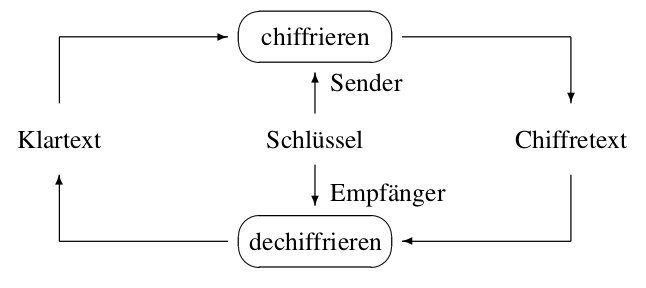
\includegraphics[scale=0.5]{figures/ver-und-entschluesseln.png}
			\quelle{(Wätjen, 2018, S.1)}
			\label{fig:ver-und-entschluesselung}
			\caption{Symmetrische Ver- und Entschlüsselung}
		\end{minipage}
	\end{figure}\par
	Von asymmetrischer Verschlüsselung ist die Rede, wenn die Teilnehmer anstatt einen gemeinsamen Schlüssel zu haben, der im vor hinein ausgetauscht werden muss, jeder ein Schlüsselpaar, bestehend aus öffentlichem und privatem Schlüssel, besitzt.\par
	
	\subsection{RSA}
	Das \gls{rsa} Verfahren ist ein solches asymmetrisches Verschlüsselungsverfahren welches von den drei namens gebenden Mathematikern 1977 entwickelt wurde. Das \gls{rsa} Verfahren ist wohl das am häufigsten verwendete Public-Key-Kryptosystem.\par
	
	\textbf{Beispiel 1.} Die Gesprächspartner Alice und Bob, welche beide ein Schlüsselpaar besitzen, wollen miteinander kommunizieren. Alice verschlüsselt einen Nachrichtentext mit dem öffentlichen Schlüssel von Bob und sendet die verschlüsselte Nachricht an Bob. Dieser kann seinerseits mit seinem privaten Schlüssel die Nachricht entschlüsseln\footnote{Vgl. Dietmar Wätjen, 2018, S.73 f.}.\par

	\subsection{Signaturen}
	Für die Sicherstellung der Authentizität können sogenannte Signaturen verwendet werden. Das oben kurz erläuterte \gls{rsa} Verfahren kann nicht nur zum Ver- und Entschlüsseln von Nachrichten benutzt werden, sondern auch zum signieren.\par
	Dabei wird statt des öffentlichen Schlüssels, der private Schlüssel, zusammen mit einer Hashfunktion, benutzt um eine Signatur zu erzeugen. Diese kann dann mit dem öffentlichen Schlüssel des zugehörigen privaten Schlüssels verifiziert werden.\par
	
	\textbf{Beispiel 2.} Bob möchte eine Nachricht an Alice schicken und sichergehen, dass diese auf dem Weg nicht verändert wurde. Er verwendet seinen privaten Schlüssel und wendet diesen auf eine Nachricht an um eine Signatur zu erzeugen. Beides übermittelt er an Alice. Mit dem öffentlichen Schlüssel von Bob kann die fehlerfreie Übertragung der Nachricht verifiziert werden.\par
	
	Eine Hashfunktion ist eine Einwegfunktion welche auch zur Signierung verwendet werden kann. Bei solch einer Funktion wird ein Eingangswert auf eine kryptische Zeichenfolge abgebildet. Dies wird sehr oft bei Passwörtern verwendet um diese nicht Umkerbar aufzubewahren.\par

	\subsection{HTTP Signaturen}
	Eine \textit{HTTP Signatur} wird verwendet um die Authentizität sicherzustellen. Diese wird als Wert einer \glqq Signature\grqq~Kopfzeile eingetragen und besteht aus mehreren Teilen:
	\begin{itemize}
		\item \textit{\textbf{keyId}}="https://example.org/activitypub/users/lea\#main-key"
		\item \textit{\textbf{algorithm}}="rsa-md4"
		\item \textit{\textbf{headers}}="(request-target) date host content-type"
		\item \textit{\textbf{signature}}="DHeEH0Okmtf1ec/lbM1/F5FiLVfQfbWuoFf9t/TzNZiZ7ak"
	\end{itemize}
	Über die \textit{keyId}, was eine Referenz auf einen Schlüssel darstellt, kann der öffentliche Schlüssel angefragt werden. Dies wird beim verifizieren einer Signatur benötigt um die übertragenen Daten auf ihre Authentizität hin zu prüfen.\par
	
	Welcher Hashing-Algorithmus bei der Erstellung verwendet wurde, kann über das \textit{algorithm} Feld der Signatur nachgeschlagen werden. Zudem muss der Algorithmus bei Erstellung in dieses Feld zum Nachschlagen eingetragen werden.\par
	
	Um die eigentliche Signatur zu erzeugen werden die in \textit{headers} angegebenen Kopfzeilen der HTTP Anfrage verwendet. Somit kann eingeschränkt werden welche Metadaten in die Signierung einfließen.\par
	
	Die bei der Signierung mit gegebenem Hashing-Algorithmus und Kopfzeilen erzeugte Signatur wird in das \textit{signature} Feld der HTTP Signatur eingetragen sowie die HTTP Signatur an sich als \glqq Signature\grqq~Kopfzeile der HTTP Anfrage gesetzt.\cite{http-signature}\par
}
		
\section{ActivityPub Standard}
\iflanguage{english}{
}{
	Der ActivityPub Standard wurde am 23 Januar 2018 von der \gls{w3c} empfohlen\cite{activityPub} und von einer Arbeitsgruppe des \gls{w3c}, der \gls{swwg}\cite{socialWg,pushSocialWeb}, entwickelt. Diese Gruppe war vom 21. Juli 2014 bis zum 13 Februar 2018 aktiv\cite{socialWg} und entwickelte unter anderem ActivityPub, \gls{asc}\cite{activityStreamsCore} und \gls{asv}\cite{activityStreamsVocabulary}. Die \gls{swwg} war eine Arbeitsgruppe des \gls{w3c} mit dem Ziel neue Protokolle, Vokabulare und \gls{api}'s zu definieren für den Zugriff auf soziale Inhalte der sogenannten \gls{owp}\cite{social-wg-charter}.\par
	
	ActivityPub definiert zwei Protokollschichten, sowie Konzepte, Sammlungen und Interaktionen für dezentrale soziale Netzwerke. Eine Protokollschicht ist das Client-zu-Server Protokoll (Social API), um Clients den Zugriff auf die neusten an sie gesendeten Inhalte zu ermöglichen sowie zum entgegennehmen von Anfragen die vom Client abgesetzt wurden\cite{activityPub}.\par 
	\begin{figure}[h]
		\begin{minipage}{\textwidth}
			\centering
			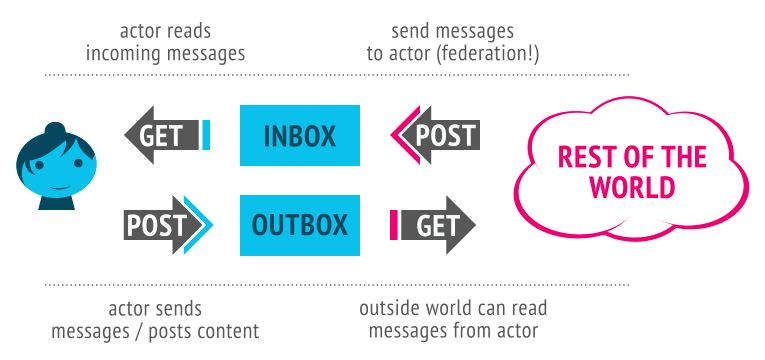
\includegraphics[scale=0.55]{figures/client-server-federated.png}
			\quelle{ActivityPub 2018 - Overview}
			\label{fig:client-server-federated}
			\caption{Schnittstellen des ActivityPub Protokolls}
		\end{minipage}
	\end{figure}\par
	Die zweite Protokollschicht besteht aus dem förderierten Server-zu-Server Protokoll (Federation Protocol), welches den einzelnen Instanzen von dezentralen sozialen Netzwerken den Austausch von Inhalten untereinander gestattet. ActivityPub setzt auf bereits bestehende Empfehlungen des \gls{w3c} auf, welche teilweise auch von der \gls{swwg} entwickelt wurden wie z. B. \gls{asc} und \gls{asv}\cite{activityPub}. Die zwei Protokollschichten können unabhängig voneinander implementiert werden.\par
	
	Auch andere Technologien wie \gls{JSON-LD} werden verwendet um die Erweiterbarkeit zu gewährleisten. Über neue Ontologien und Vokabulare können weitere syntaktische Definitionen und semantische Beschreibungen zu den bestehenden hinzugefügt werden\cite{activityPub}. Diese Vokabulare können im Kontext des \gls{JSON-LD} Objektes, angegeben werden. Bei ActivityPub wird das \gls{AS2} Vokabular verwendet welches durch \gls{asv} erweitert wird.\par
}
\subsection{
	\iflanguage{english}{Elements of the protocol}{Bestandteile des Protokolls}
}
\iflanguage{english}{}{
	Die Hauptbestandteile des ActivityPub Standards sind die folgenden:\par
	\begin{itemize}
		\item Aktoren
		\item Objekte
		\item Sammlungen
		\item Aktivitäten
	\end{itemize}
	In ActivityPub werden Benutzer als \glqq Aktoren\grqq(actors) dargestellt. Diese können nicht nur Personen, sondern auch Applikationen, Organisationen, Gruppen und Services sein\cite{activityStreamsCore}. Jedes Aktoren Objekt muss eine \glqq Inbox\grqq~und \glqq Outbox\grqq, welche geordnete Sammlungen sein müssen, sowie eine ID und ein Typ besitzen\cite{activityPub}. Die ID muss global einzigartig sein. Dies kann garantiert werden durch eine Domänen und Protokoll bezogene URI oder IRI wie z. B. \glqq https://example.org/users/alice\grqq oder \glqq https://example.org/users/álìcê\grqq. Der Typ eines Aktor (z. B. "type": "Person") kann variieren zwischen den fünf oben genannten.\par
	\begin{figure}[h]
		\begin{minipage}{\textwidth}
			\centering
			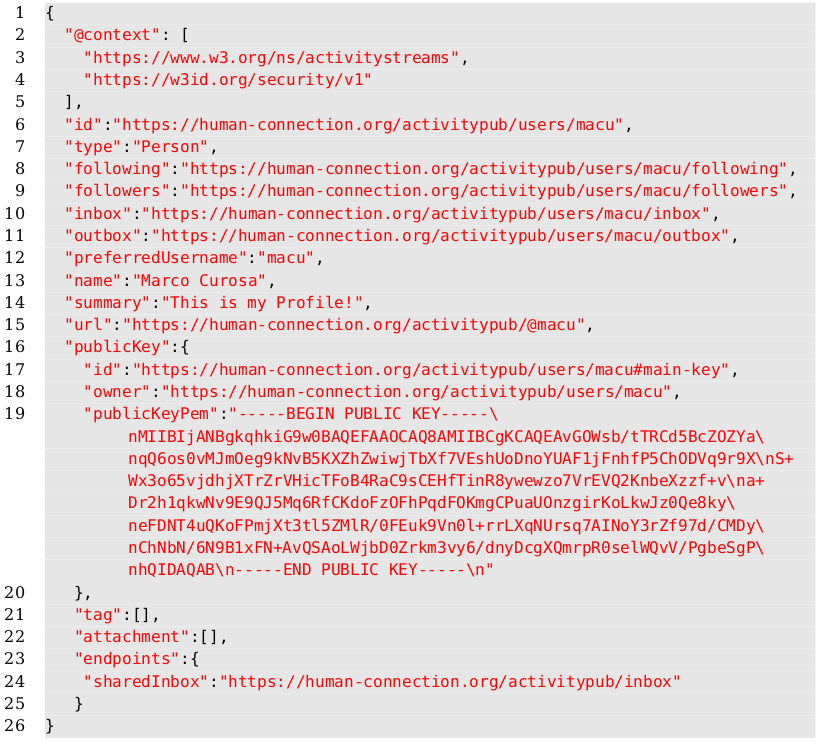
\includegraphics[scale=0.5]{figures/actor.png}
			\label{fig:actor}
			\caption{Beispiel Aktoren Objekt}
		\end{minipage}
	\end{figure}\par
}
\subsection{
	\iflanguage{english}{Related standards and components}{Zugehörige Standards und Komponenten}
}
\iflanguage{english}{}{
	ActivityPub benutzt die ActivityStreams Daten Syntax und das Vokabular. Zusätzlich kann ein weiteres Sicherheitsvokabular\footnote{Eine Ontologie die Sicherheitsaspekte definiert wie öffentliche Schlüssel, Signaturen u.v.m.} benutzt werden um Definitionen zum Bereitstellen eines öffentlichen Schlüssels, Signaturen sowie Verschlüsselten Inhalten u.v.m. zu haben. Am 22 April 2016 hat die \glqq W3C Community Group\grqq~ einen Entwurfsbericht herausgebracht. Durch diesen wird neue Syntax und Semantik definiert um Internet basierten Applikationen das Verschlüsseln, Entschlüsseln sowie digitale Signieren und Verifizieren von verlinkten Daten (Linked Data) zu ermöglichen. Es enthält auch Vokabeln für die Erstellung und Verwaltung einer dezentralen Public-Key-Infrastruktur über das Internet\cite{security-vocab-linked-data}. Ein Anwendungsfall ist das holen des öffentlichen Schlüssels eines Nutzers, über dessen Aktoren Objekt, um eine von Nutzer gesendete Nachricht zu verifizieren.\par
	
	\glqq \gls{AS2}\grqq~beinhaltet Modelle für Aktoren, Aktivitäten, Intransitiven Aktivitäten, Objekte, Links, Sammlungen, Natürliche Sprachwerte (Strings) und für Internationalisierung. Das Kernvokabular von \gls{AS2} wird durch \gls{asv} erweitert. Dazu gehören verschiedene Aktivitätstypen wie z.B. \glqq Accept\grqq,\glqq Add\grqq,\glqq Remove\grqq,\glqq Delete\grqq~und \glqq Create\grqq\footnote{\href{https://www.w3.org/TR/activitystreams-vocabulary/}{activity-types https://www.w3.org/TR/activitystreams-vocabulary/}}, um Aktorentypen wie \glqq Person\grqq, \glqq Application\grqq~und \glqq Group\grqq\footnote{\href{https://www.w3.org/TR/activitystreams-vocabulary/}{actor-types https://www.w3.org/TR/activitystreams-vocabulary/}} sowie um verschiedenste Objekttypen wie \glqq Article\grqq, \glqq Event\grqq, \glqq Note\grqq~und \glqq Relationship\grqq\footnote{\href{https://www.w3.org/TR/activitystreams-vocabulary/}{object-types https://www.w3.org/TR/activitystreams-vocabulary/}}.\par
	
	\gls{JSON-LD} ist eine Erweiterung des JSON Formates um verlinkte Daten zu Repräsentieren. JSON an sich, ist ein Format welches im Web häufig Anwendung findet um Daten auszutauschen. Im Kern sind \gls{AS2} auch \gls{JSON-LD} Objekte. Der \gls{AS2} Kontext definiert verschiedene Klassen und Eigenschaften, von denen nicht alle benutzt werden. Typische Klassen sind \glqq Activity\grqq, \glqq Link\grqq~und \glqq OrderedCollection\grqq. Ein Beispiel Notiz, sowie Artikel \gls{AS2} Objekt sieht wie folgt aus:\par
	\begin{figure}[h]
		\begin{minipage}{\textwidth}
			\centering
			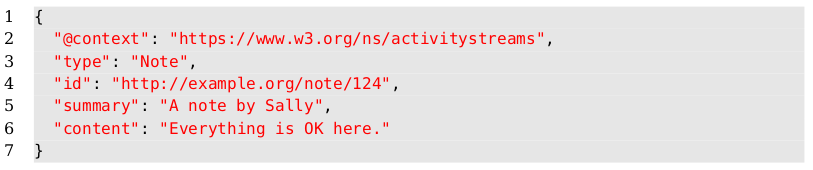
\includegraphics[scale=0.5]{figures/object-note.png}
			\label{fig:object-note}
			\caption{Beispiel Notiz Objekt}
		\end{minipage}
	\end{figure}
	\begin{figure}[h]
		\begin{minipage}{\textwidth}
			\centering
			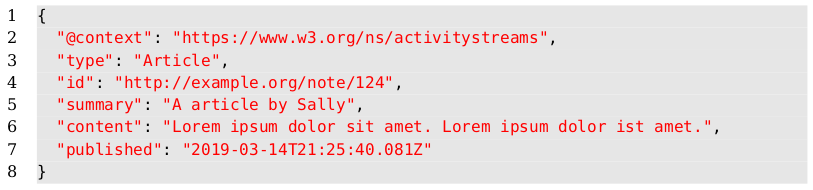
\includegraphics[scale=0.5]{figures/object-article.png}
			\label{fig:object-article}
			\caption{Beispiel Artikel Objekt}
		\end{minipage}
	\end{figure}
	% \lstinputlisting[caption={Beispiel \gls{AS2} Objekt}, label=listing::as2-object, language=JavaScript]{resources/example-as2-object.json}
}
\subsection{
	\iflanguage{english}{Authentication and data integrity}{Authentifizierung und Datenintegrität}
}
\iflanguage{english}{}{
	Für die Authentifizierung und zum sichern der Datenintegrität definiert der Standard keine Mechanismen. Es gibt allerdings \glqq Best Practices\grqq~für die Umsetzung dieser Anforderungen.\par

	Zum einen werden bei der Client-zu-Server Authentifizierung \glqq OAuth 2.0 Bearer Tokens\grqq~benutzt, zum anderen auf der Server Seite \glqq HTTP\grqq~oder \glqq Linked Data Signatures\grqq zur Sicherstellung der Datenintegrität.\par

	Bei\glqq OAuth 2.0 Bearer Tokens\grqq~handelt es sich um eine Methode um auf geschützte Ressourcen zugreifen zu können\cite{oauth2}. ActivityPub nutzt diese für jegliche Interaktionen mit dem Server.\par
	
	\glqq Die Datenintegrität umfasst Maßnahmen damit geschützte Daten während der Verarbeitung oder Übertragung nicht durch unautorisierte Personen entfernt oder verändert werden können. Sie stellt die Konsistenz, die Richtigkeit und Vertrauenswürdigkeit der Daten während deren gesamten Lebensdauer sicher und sorgt dafür, dass die relevanten Daten eines Datenstroms rekonstruierbar sind\grqq\cite{data-integrity}.\par
	
	Um sicherzustellen das HTTP Anfragen beim Transport nicht verändert wurden, können HTTP Signaturen verwendet werden. Diesen verwenden einen kryptografischen Algorithmus um aus ausgewählten Kopfzeilen einer HTTP Anfrage einen kryptischen Zeichenfolge zu generieren. Auf der Empfängerseite kann die Zeichenfolge mit mitgelieferten und auch nachschlagbaren Information verifiziert werden.\par
	
	Wenn ein Objekt nicht nur vom Client zum Server gesendet, sondern auch zwischen Servern untereinander weitergeleitet werden soll wird zum Sicherstellen der Datenintegrität ein anderes Verfahren benötigt als HTTP Signaturen. Die \glqq Best Practices\grqq~empfehlen für solche Fälle \glqq Linked Data Signatures\grqq. Der größte Unterschied zwischen HTTP Signaturen und \glqq Linked Data Signatures\grqq~besteht darin, welche Daten zum Erstellen der Signatur verwendet werden. Bei HTTP Signaturen sind es die Kopfzeilen. Mit \glqq Linked Data Signatures\grqq~kann auch das Objekt selbst, also der Payload einer HTTP Anfrage, anstatt nur die Kopfzeilen, zum signieren verwendet werden.\par
}

%%% LaTeX2e class for student theses
%% sections/content.tex
%%
%% Karlsruhe University of Applied Sciences
%% Faculty of  Computer Science and Business Information Systems
%% Distributed Systems (vsys)
%%
%% Prof. Dr. Christian Zirpins
%% christian.zirpins@hs-karlsruhe.de
%%
%%
%% Version 0.2, 2017-11-15
%%
%% --------------------------------------------------------
%% | Derived from sdqthesis by Erik Burger burger@kit.edu |
%% --------------------------------------------------------

\chapter{Analyse bestehender Ansätze}
\label{ch:analysis_given_approachs}

\section{Vergleich bestehender Implementierungen}
\section{Verwandte Protokolle}
	\subsection{OStatus}
	\label{subsec:ostatus}
	\begin{itemize}
		\item OStatus
		\item Diaspora Federation
	\end{itemize}
%% LaTeX2e class for student theses
%% sections/content.tex
%%
%% Karlsruhe University of Applied Sciences
%% Faculty of  Computer Science and Business Information Systems
%% Distributed Systems (vsys)
%%
%% Prof. Dr. Christian Zirpins
%% christian.zirpins@hs-karlsruhe.de
%%
%%
%% Version 0.2, 2017-11-15
%%
%% --------------------------------------------------------
%% | Derived from sdqthesis by Erik Burger burger@kit.edu |
%% --------------------------------------------------------

\chapter{Entwurf einer Lösung für sichere Server-zu-Server Interaktion mit ActivityPub}
Zu Beginn dieses Kapitels sollte sich die Frage gestellt werden wie die Architektur sicher gestaltet wird. 

Eine Trennung der ActivityPub Komponenten in einen eigenen Service würde für eine isolierbare Ausführung sorgen. Es
\section{Entwurfsentscheidung}
\section{Technische Architektur}
	\begin{figure}[h]
		\centering
		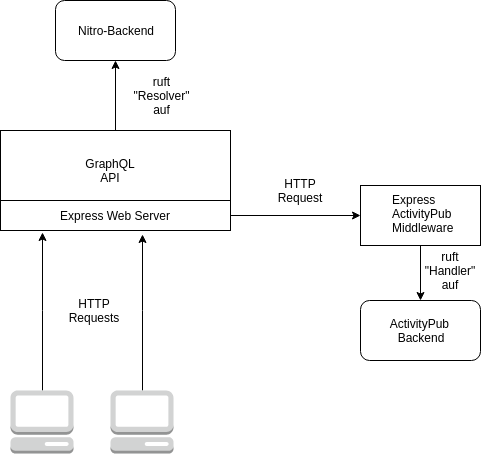
\includegraphics[scale=0.5]{figures/technische-architektur-activitypub.png}
		\label{technische-architektur-activitypub}
		\caption{Technische Architektur ActivityPub}
	\end{figure}
	Der technischen Architektur liegt das Express Middleware Framework zugrunde. Der ActivityPub Service wird als Express Middleware, sowie als allein stehender Express Web Server implementiert. Bei der letzteren Variante wird anstatt die Middleware in ein bestehenden Express Server zu integrieren, ein eigener Express Server gestartet.\\
	
	In der oben gezeigten Abbildung wurde der ActivityPub Service in einen bestehenden Express Server einer GraphQL API integriert.\\
	
	Benutzer der API kommunizieren mit dem Web Server über das HTTP Protokoll. Der Web Server leitet die Anfragen dann an den entsprechenden Router weiter, welcher wiederum den Anfrage Inhalt transformiert und \glqq Handler\grqq~Funktionen des ActivityPub Service mit entsprechenden Parametern aufruft.\\
	
	\begin{figure}[h]
		\begin{minipage}{\textwidth}
			\centering
			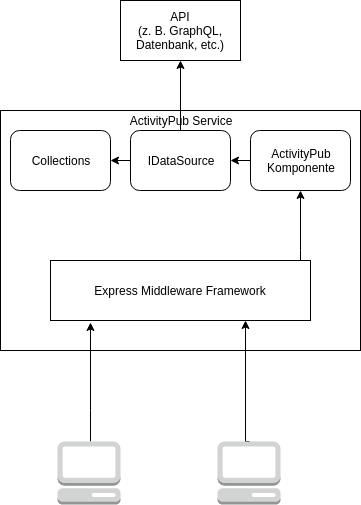
\includegraphics[scale=0.5]{figures/Technische-Architektur-standalone.png}
			\label{technische-architektur-standalone}
			\caption{Technische Architektur als allein stehender Server}
		\end{minipage}
	\end{figure}

	Die obige Abbildung zeigt eine detailliertere Variante des ActivityPub Service Diagramms aus Abb. 4.1.\\
	Es wird außerdem ersichtlich, dass, um eine maßgeschneiderte Version für ein weiteres Projekt zu erstellen, das Interface IDataSource implementiert werden muss.\\ 
	Sonst wird bei der Architektur weitestgehend darauf Wert gelegt, dass die meisten ActivityPub konformen Inhalte \glqq on the fly\grqq generiert werden können. Damit wird versucht für weitere Projekte die auf diesem Prototypen aufbauen wollen einen einfachen Einstieg zu bieten um andere Datenbanken o.ä. anbinden zu können.
%% LaTeX2e class for student theses
%% sections/content.tex
%%
%% Karlsruhe University of Applied Sciences
%% Faculty of  Computer Science and Business Information Systems
%% Distributed Systems (vsys)
%%
%% Prof. Dr. Christian Zirpins
%% christian.zirpins@hs-karlsruhe.de
%%
%%
%% Version 0.2, 2017-11-15
%%
%% --------------------------------------------------------
%% | Derived from sdqthesis by Erik Burger burger@kit.edu |
%% --------------------------------------------------------

\chapter{Implementierung eines ActivityPub Prototyps}
Die IDataSource Implementierung wird für das Unternehmen angefertigt in der die Bachelor Thesis bearbeitet wird. Im Falle man möchte den Service mit einer anderen Datenquelle versorgen, kann das IDataSource Interface implementiert und so angepasst werden, dass eine andere Datenbank Verwendung findet.\\

\begin{figure}[h]
	\begin{minipage}{\textwidth}
		\centering
		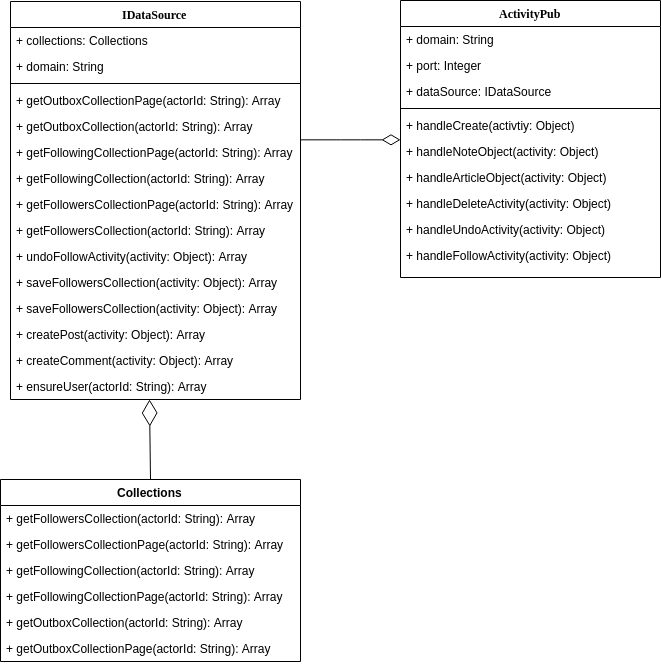
\includegraphics[scale=0.5]{figures/klassendiagramm-activitypub.png}
		\label{klassendiagramm-activitypub}
		\caption{Hauptkomponenten des förderierten Servers}
	\end{minipage}
\end{figure}
\section{Server-zu-Server Protokoll}
%% LaTeX2e class for student theses
%% sections/evaluation.tex
%%
%% Karlsruhe University of Applied Sciences
%% Faculty of  Computer Science and Business Information Systems
%% Distributed Systems (vsys)
%%
%% Prof. Dr. Christian Zirpins
%% christian.zirpins@hs-karlsruhe.de
%%
%%
%% Version 0.2, 2017-11-15
%%
%% --------------------------------------------------------
%% | Derived from sdqthesis by Erik Burger burger@kit.edu |
%% --------------------------------------------------------

\chapter{Evaluation}
\label{ch:Evaluation}

\section{Anwendungsbeispiel}
\section{(Performanzmessungen)}
Die Performanzmessung wurde in der NodeJs Laufzeitumgebung mit der Version 10.15.3 durchgeführt unter Zuhilfenahme der internen process.hrtime() Funktion. Diese wird vor und nach dem Erstellen sowie Verifizieren aufgerufen. Die Rückgabe des zweiten Aufrufs nach der jeweiligen Funktion enthält die Differenz zum ersten Aufruf in Nanosekunden.
\begin{table}
	\begin{tabularx}{\textwidth}{p{0.15\textwidth}|r|X|X|r}
		& rsa-md4 & rsa-md5 & rsa-sha256 & rsa-sha512\\
		\hline
		Testlauf 1& 24.254 ms& 24.123 ms& 24.171 ms& 24.173 ms\\
		Testlauf 2& 22.833 ms& 23.006 ms& 23.626 ms& 22.948 ms\\
		Testlauf 3& 27.186 ms& 23.113 ms& 22.873 ms& 22.781 ms\\
		Testlauf 4& 23.630 ms& 24.256 ms& 22.597 ms& 22.667 ms\\
		Testlauf 5& 25.012 ms& 24.027 ms& 24.343 ms& 30.278 ms\\
		Testlauf 6& 30.221 ms& 23.032 ms& 22.827 ms& 22.768 ms\\
		Testlauf 7& 27.050 ms& 29.950 ms& 22.629 ms& 22.774 ms\\
		Testlauf 8& 23.630 ms& 24.282 ms& 24.625 ms& 25.495 ms\\
		Testlauf 9& 23.151 ms& 22.958 ms& 22.854 ms& 26.816 ms\\
		Testlauf 10& 22.654 ms& 24.067 ms& 23.637 ms& 23.579 ms\\
		\hline
		Arithmetisches Mittel& 25,122 ms& 24,281 ms& 23,418 ms& 24,427 ms\\
	\end{tabularx}\\
	\caption{Testergebnisse der Signatur Erstellung}
\end{table}
Beim betrachten der arithmetischen Mittel fällt auf, dass die Werte sehr nahe beieinander liegen 
\begin{table}
	\begin{tabularx}{\textwidth}{p{0.15\textwidth}|r|X|X|r}
		& rsa-md4 & rsa-md5 & rsa-sha256 & rsa-sha512\\
		\hline
		Testlauf 1& 107,177 ms& 128.993 ms& 121.406 ms& 114.669 ms\\
		Testlauf 2& 43,660 ms& 51.178 ms& 35.524 ms& 39.633 ms\\
		Testlauf 3& 32.101 ms& 32.691 ms& 30.461 ms& 32.293 ms\\
		Testlauf 4& 36.096 ms& 30.279 ms& 32.018 ms& 43.842 ms\\
		Testlauf 5& 31.869 ms& 34.882 ms& 30.877 ms& 26.555 ms\\
		Testlauf 6& 39.218 ms& 67.507 ms& 38.734 ms& 31.330 ms\\
		Testlauf 7& 40.996 ms& 39.646 ms& 45.433 ms& 27.290 ms\\
		Testlauf 8& 25.977 ms& 39.302 ms& 26.778 ms& 53.478 ms\\
		Testlauf 9& 23.641 ms& 37.833 ms& 30.485 ms& 36.284 ms\\
		Testlauf 10& 31.097 ms& 52.725 ms& 28.943 ms& 28.634 ms\\
		\hline
		Arithmetisches Mittel& 41,183 ms& 51,503 ms& 42,065 ms& 43,400 ms\\
	\end{tabularx}\\	
	\caption{Testergebnisse der Signatur Verifikation}
\end{table}

\section{Disskusion von Vor- und Nachteilen der Lösung}

%% LaTeX2e class for student theses
%% sections/conclusion.tex
%%
%% Karlsruhe University of Applied Sciences
%% Faculty of  Computer Science and Business Information Systems
%% Distributed Systems (vsys)
%%
%% Prof. Dr. Christian Zirpins
%% christian.zirpins@hs-karlsruhe.de
%%
%%
%% Version 0.2, 2017-11-15
%%
%% --------------------------------------------------------
%% | Derived from sdqthesis by Erik Burger burger@kit.edu |
%% --------------------------------------------------------
\chapter{Fazit \& Ausblick}
\todo{Im Fazit die Arbeit nochmal Zussammenfassen, blos kennt der Leser die Arbeit bereits}
\section{Fazit}
Ergebnisse, wie sind sie einzuordnen, 
\section{Ausblick}
\label{ch:Conclusion}
Da das Interface sehr groß werden kann beim hinzufügen weiterer Funktionalität könnte dieses neu Strukturiert oder aufgeteilt werden. Beispielsweise kann eine weitere Arbeit innerhalb des Interfaces Fassaden-Klassen anlegen. Es könnte sich auch ein neues Interface Design überlegt werden.\\

Die Implementierung beinhaltet zur Authentifizierung der Server untereinander sowie zur Sicherstellung der Datenintegrität Funktionalität zum Erstellen und Verifizieren von HTTP-Signaturen. Eine weitere Arbeit kann mit einer Implementierung der Funktionalität zum Signieren und Verifizieren von unterschiedlichen \textit{Linked Data} Signatur Typen und einer Performanz-Messung dieser Implementierung auf diese Arbeit aufbauen.\\

Zur Erweiterung der Funktionalität des Frameworks können weitere Werkzeugklassen sowie Logik zum Verarbeiten zusätzlicher Aktivitäten und Objekte hinzugefügt werden. Das Framework enthält bis dato keine seitens des Standards definierten Aktivitäten zum hinzufügen zu und entfernen von Aktivitäten aus Sammlungen (Add, Remove). Auch weitere Objekttypen wie \textit{Audio} oder \textit{Video} können hinzugefügt werden\footnote{siehe \url{https://www.w3.org/TR/activitystreams-vocabulary/}, 3.3}.\\

Auch eine Komponente zum Schutz vor förderierten \textit{denial-of-service} Attacken des förderierten Servers könnte implementiert werden. Der Nutzerinhalt von Objekten kann außerdem so bereinigt werden, dass kein \textit{cross-site-scripting} stattfinden kann.\\

\todo{Zitieren bei Nummerierung bleiben; Mit Absatz dahinter}
\todo{21.04}


%% --------------------
%% |   Bibliography   |
%% --------------------

%% Add entry to the table of contents for the bibliography
\printbibliography[heading=bibintoc]


%% ----------------
%% |   Appendix   |
%% ----------------
\appendix
%% LaTeX2e class for student theses
%% sections/apendix.tex
%%
%% Karlsruhe University of Applied Sciences
%% Faculty of  Computer Science and Business Information Systems
%% Distributed Systems (vsys)
%%
%% Prof. Dr. Christian Zirpins
%% christian.zirpins@hs-karlsruhe.de
%%
%%
%% Version 0.2, 2017-11-15
%%
%% --------------------------------------------------------
%% | Derived from sdqthesis by Erik Burger burger@kit.edu |
%% --------------------------------------------------------



\iflanguage{english}
{\chapter{Appendix}}    % english style
{\chapter{Anhang}}      % german style
\label{chap:appendix}


%% -------------------
%% | Example content |
%% -------------------
\section{First Appendix Section}
\label{sec:appendix:FirstSection}

\setcounter{figure}{0}

\begin{figure} [ht]
  \centering
  \missingfigure{A figure}
  \caption{A figure}
  \label{fig:anotherfigure}
\end{figure}


\dots
%% ---------------------
%% | / Example content |
%% ---------------------


\end{document}
